\documentclass[border=3mm]{standalone}
\usepackage{tikz}
\usepackage{amsmath}
\usepackage{mathptmx}
\usetikzlibrary{calc}

\begin{document}
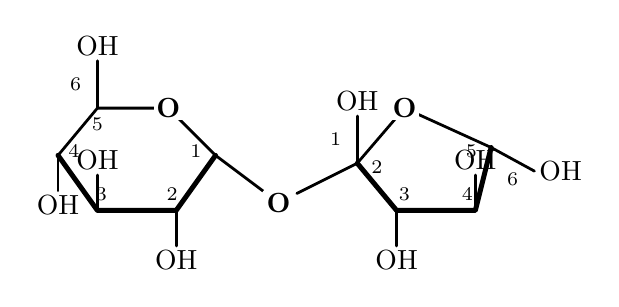
\begin{tikzpicture}[line cap=round, line join=round, line width=1.0pt, font=\fontsize{10}{12}\selectfont]
    % Vòng 1: alpha-glucopyranose (vòng 6 cạnh)
    \begin{scope}[shift={(0,0)}]
        \coordinate (gO) at (0.8, 0.7);
        \coordinate (g1) at (1.4, 0.1);
        \coordinate (g2) at (0.9, -0.6);
        \coordinate (g3) at (-0.1, -0.6);
        \coordinate (g4) at (-0.6, 0.1);
        \coordinate (g5) at (-0.1, 0.7);

        % Các cạnh vòng (cạnh đáy vẽ đậm hơn)
        \draw (g5) -- (gO) -- (g1);
        \draw[line width=1.8pt] (g1) -- (g2) -- (g3) -- (g4);
        \draw (g4) -- (g5);

        % Số thứ tự carbon
        \node at ($(g1)+(-0.25,0.05)$) {\scriptsize 1};
        \node at ($(g2)+(-0.05,0.2)$) {\scriptsize 2};
        \node at ($(g3)+(0.05,0.2)$) {\scriptsize 3};
        \node at ($(g4)+(0.2,0.05)$) {\scriptsize 4};
        \node at ($(g5)+(0.0, -0.2)$) {\scriptsize 5};

        % Cầu oxy
        \node (Oat) at (gO) [fill=white, inner sep=1pt] {\textbf{O}};

        % Nhóm thế
        \draw (g5) -- ($(g5)+(0,0.6)$) node[above=-2pt] {$\mathrm{OH}$} node[left=2pt, midway] {\scriptsize 6};
        \draw (g4) -- ($(g4)+(0,-0.45)$) node[below=-2pt] {$\mathrm{OH}$};
        \draw (g3) -- ($(g3)+(0,0.45)$) node[above=-2pt] {$\mathrm{OH}$};
        \draw (g2) -- ($(g2)+(0,-0.45)$) node[below=-2pt] {$\mathrm{OH}$};

        % Liên kết glycosidic ở g1 chúc xuống
        \coordinate (linkO) at (2.2, -0.5);
        \draw (g1) -- (linkO) node[midway, below=2pt] {};
    \end{scope}

    % Cầu oxy giữa hai gốc
    \node (bridgeO) at (2.2, -0.5) [circle, fill=white, inner sep=1pt] {\textbf{O}};

    % Vòng 2: beta-fructofuranose (vòng 5 cạnh)
    \begin{scope}[shift={(4.0,0)}]
        \coordinate (fO) at (-0.2, 0.7);
        \coordinate (f2) at (-0.8, 0.0);
        \coordinate (f3) at (-0.3, -0.6);
        \coordinate (f4) at (0.7, -0.6);
        \coordinate (f5) at (0.9, 0.2);

        \draw (f5) -- (fO) -- (f2);
        \draw[line width=1.8pt] (f2) -- (f3) -- (f4) -- (f5);

        % Số thứ tự
        \node at ($(f2)+(0.25, -0.05)$) {\scriptsize 2};
        \node at ($(f3)+(0.1, 0.2)$) {\scriptsize 3};
        \node at ($(f4)+(-0.1, 0.2)$) {\scriptsize 4};
        \node at ($(f5)+(-0.25, -0.05)$) {\scriptsize 5};

        \node (Ofruct) at (fO) [fill=white, inner sep=1pt] {\textbf{O}};

        % Nhóm thế ở f2
        \draw (f2) -- ($(f2)+(0,0.6)$) node[above=-2pt] {$\mathrm{OH}$} node[left=2pt, midway] {\scriptsize 1};
        % Nối từ cầu oxy vào f2
        \draw (bridgeO) -- (f2);

        % Nhóm thế ở f3, f4, f5
        \draw (f3) -- ($(f3)+(0,-0.45)$) node[below=-2pt] {$\mathrm{OH}$};
        \draw (f4) -- ($(f4)+(0,0.45)$) node[above=-2pt] {$\mathrm{OH}$};
        \draw (f5) -- ($(f5)+(0.55,-0.3)$) node[right=-2pt] {$\mathrm{OH}$} node[below=1pt, midway] {\scriptsize 6};
    \end{scope}
\end{tikzpicture}
\end{document}
